\documentclass{beamer}
\usepackage[english]{babel}
\usepackage[utf8]{inputenc}
\usepackage{verbatim}
\usepackage{graphicx}

\begin{document}

\title{Telepathy Framework Intro}
\author{Maksim Melnikau (max\_posedon)}
\institute{Linux Mobile hobbyist\\World of Tanks developer}
\date{\today}
\frame{\titlepage}

\frame{
    \frametitle{Conceptual example}
    \begin{figure}[htb]
    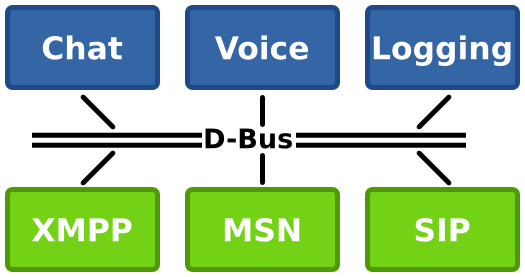
\includegraphics[width=\textheight]{tao.png}
    \end{figure}
}

\frame{
    \frametitle{Desktop applications}
    \begin{itemize}
    \item Empathy
    \item kde-telepathy
    \end{itemize}
}

\frame{
    \frametitle{Mobile devices}
    \begin{itemize}
    \item N770 / N800 / N810
    \item N900
    \item N9 ( N950 )
    \end{itemize}
}

\frame{
    \frametitle{Most popular protocols}
    \begin{itemize}
    \item Gabble: for XMPP, including support for Jingle
    \item Butterfly: for Windows Live Messenger
    \item Idle: for Internet Relay Chat
    \item Salut: for the link-local XMPP protocol
    \item Haze: for accessing protocols supported by libpurple, the library used by the Pidgin messaging client.
    \item Rakia: for the Session Initiation Protocol (SIP), using Nokia's open source Sofia-SIP library
    \end{itemize}
}

\frame{
    \frametitle{telepathy libraries}
    \begin{itemize}
    \item telepathy-glib
    \item telepathy-qt
    \item telepathy-python
    \end{itemize}
}

\frame{
    \frametitle{Questions and Answers}
    \begin{itemize}
    \item email: maxposedon@gmail.com
    \end{itemize}
}

\end{document}
